\begin{figure}[htbp]
\centering
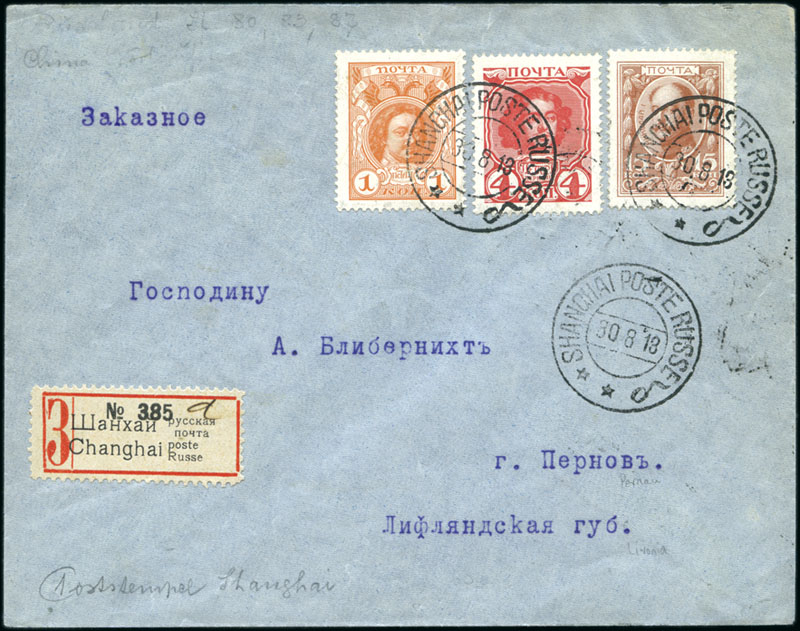
\includegraphics[width=.95\textwidth]{../russian-post-offices-in-china/10080.jpg}
\caption{
 10080 SHANGHAI: 1913 Cover sent registered to Pernov with Romanov 1k,
 4k and 15k tied by Shanghai 30.8.13 cds (T\&S type 6B), with bilingual reg'd 
 label adjacent, Pernov bs, a rare franking as the Romanov issue was not 
 available in the Russian P.O.s in China, but was accepted when supplied 
 by the customer.
\euro 400.00
}  
\end{figure}

\begin{figure}[htbp]
\centering
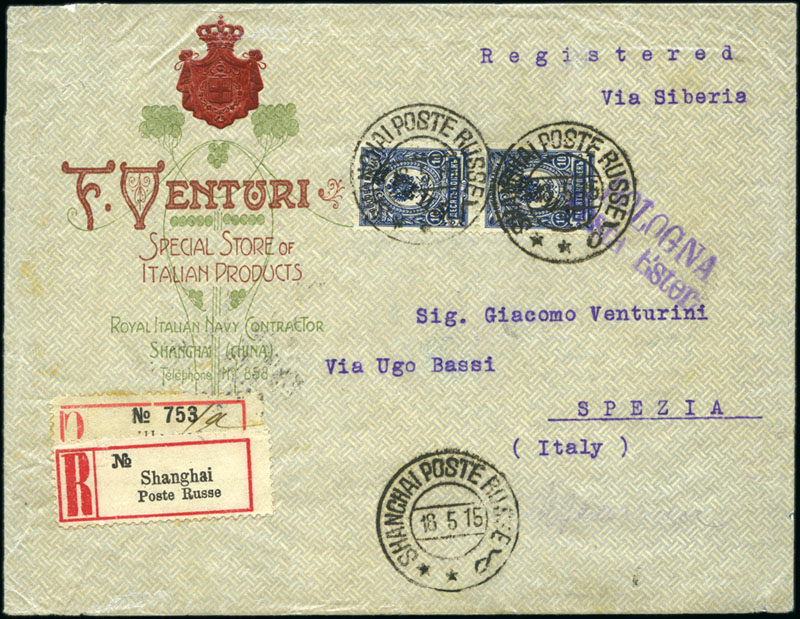
\includegraphics[width=.95\textwidth]{../russian-post-offices-in-china/10081.jpg}
\caption{
10081SHANGHAI: 1915 Advertising cover sent registered to Italy with "KITAI" 10k
vert. pair tied by Shanghai 18.5.15 cds (T\&S type 6B), with reg'd labels in 
Cyrillic and French adjacent with Bologna two-line hs, reverse with Moscow 
censor hs and Spezia arrival, attractive and unusual cover.
\euro 300.00  
}  
\end{figure}
            
\begin{figure}[htbp]
\centering
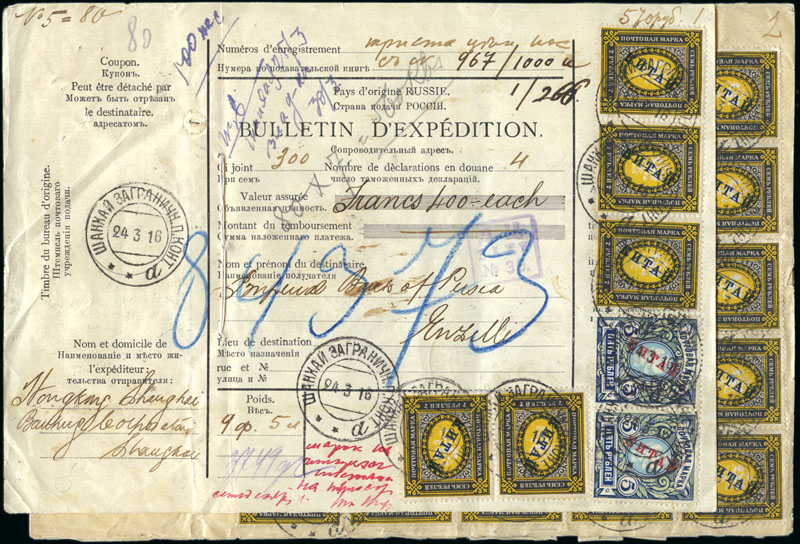
\includegraphics[width=.95\textwidth]{../russian-post-offices-in-china/10082.jpg}
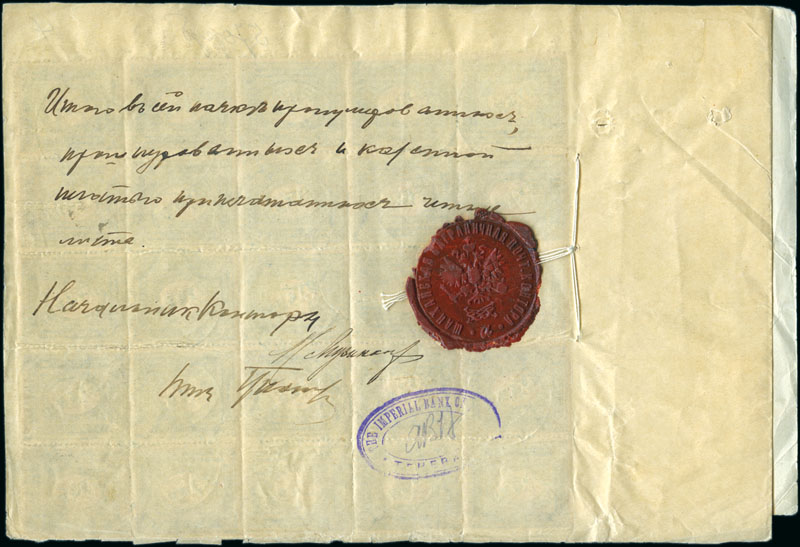
\includegraphics[width=.95\textwidth]{../russian-post-offices-in-china/10082-1.jpg}
\caption{
10082	SHANGHAI: 1916 Despatch document (Bulletin D'Exp\'edition) for consignment
to Persia, franked with eighty "KITAI" 7R (incl. three sheets of twenty-five) 
and a pair of 5R paying the 570R charge, cancelled by Shanghai 24.3.16 cds (
T\&S type 8A), reverse with "Shanghai Post Office Abroad" Imperial Eagle 
wax seal, examined by censor at Baku, a fantastic franking

Provenance: ex Mizuhara
\euro 3,000.00 
}  
\end{figure}

\begin{figure}[htbp]
\centering
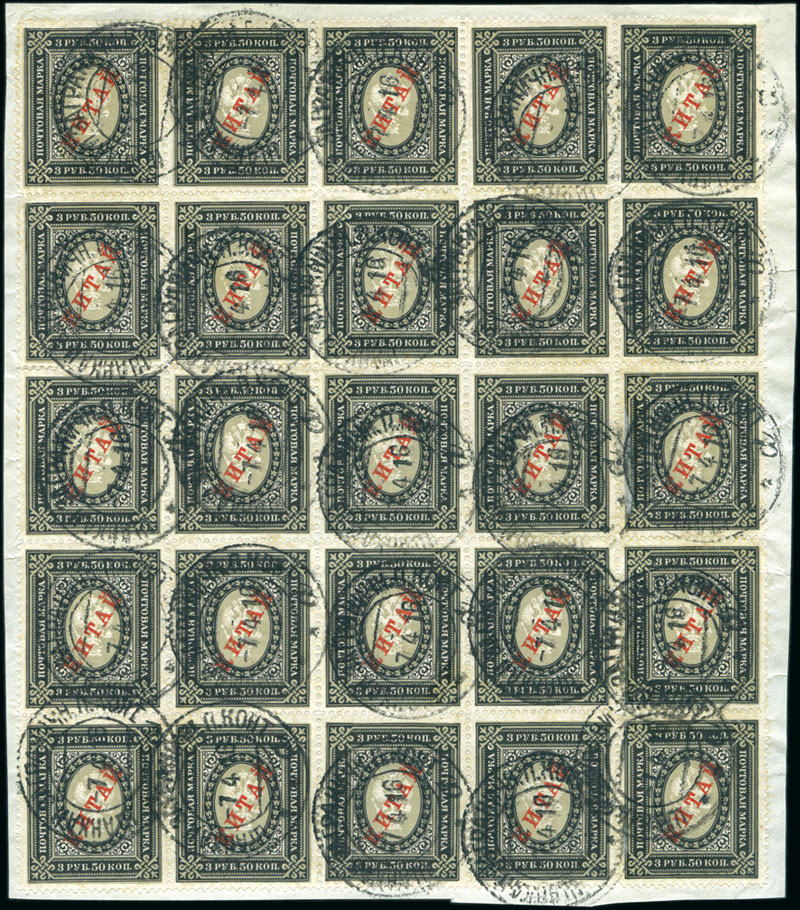
\includegraphics[width=.95\textwidth]{../russian-post-offices-in-china/10083.jpg}
\caption{
10083		ZoomSHANGHAI: 3R50k in sheet of 25 originally 
attached to a parcel card, with each stamp cancelled by Shanghai
7.4.16 cds (T\&S type 8a), very fine and rare multiple
\euro 200.00 
}  
\end{figure}            
            
\begin{figure}[htbp]
\centering
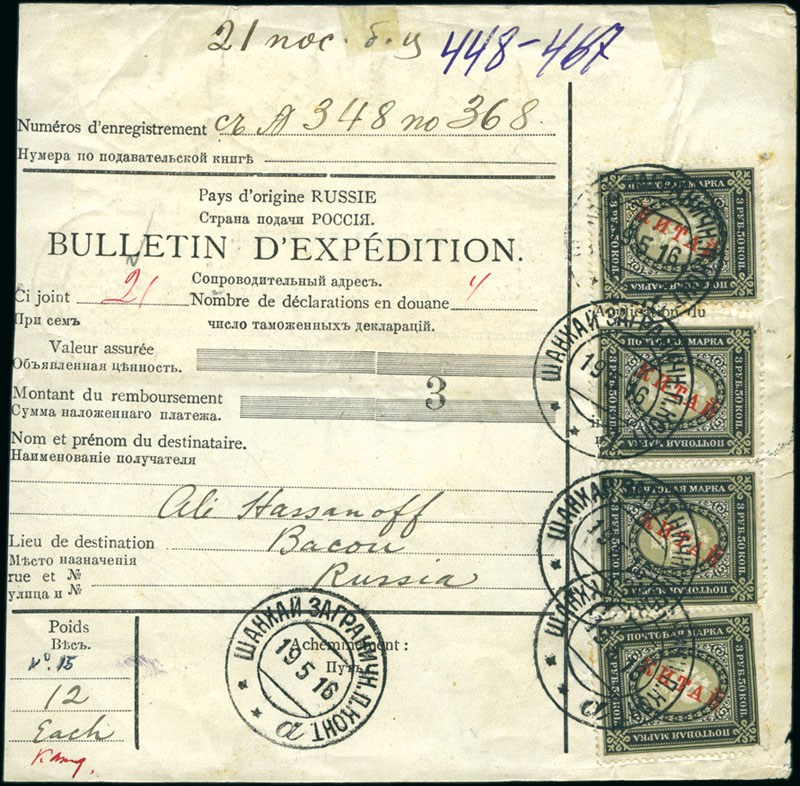
\includegraphics[width=.95\textwidth]{../russian-post-offices-in-china/10084.jpg}
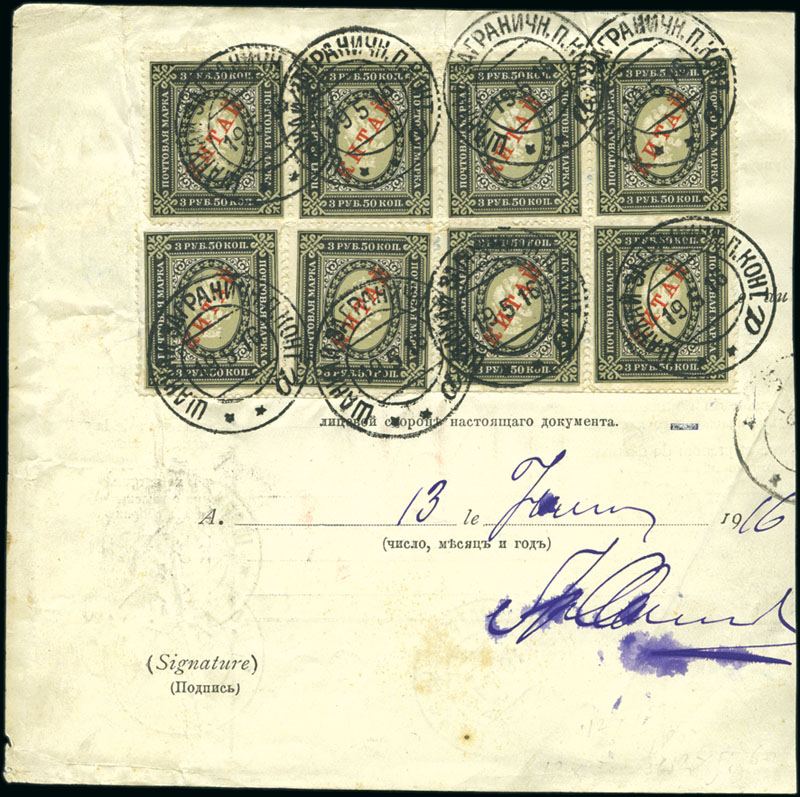
\includegraphics[width=.95\textwidth]{../russian-post-offices-in-china/10084-1.jpg}
\caption{
10084		ZoomSHANGHAI: 1916 Dispatch document (Bulletin D'Exp\'edition) for 
21 packages sent to Baku, with charges paid by twelve "KITAI" 3R50k on 
front and back tied by Shanghai 19.5.16 cds (T\&S type 8A), scarce.
\euro 400.00  
}  
\end{figure} 


\begin{figure}[htbp]
\centering
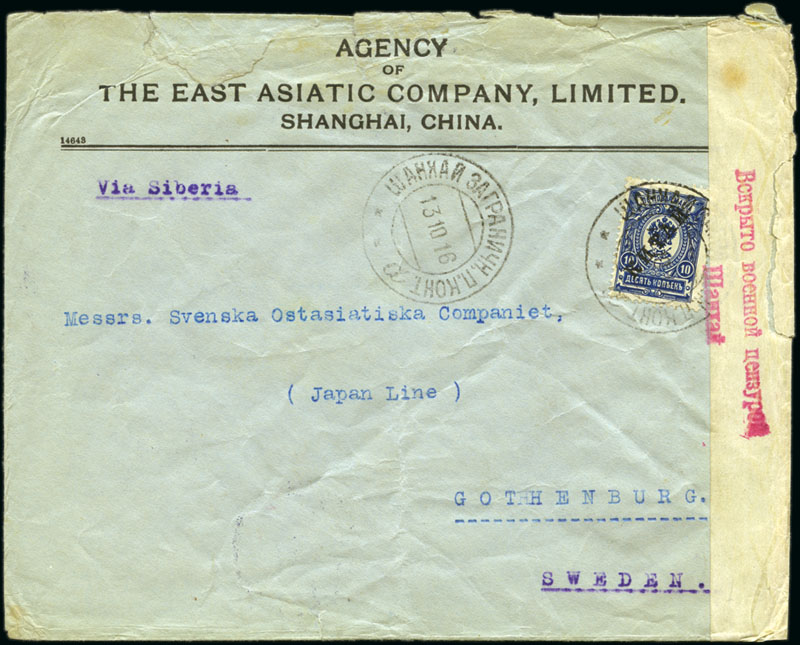
\includegraphics[width=.95\textwidth]{../russian-post-offices-in-china/10085.jpg}
\caption{
 10085	SHANGHAI: 1916 Cover to Sweden with "KITAI" 10k tied by Shanghai 13.10.16 
 cds (T\&S type 8A), opened and resealed by censor in Shanghai with paper 
 seal and two-line "Opened by Military Censor / Shanghai" hs in Cyrillic 
 (Speeckaert type 3 with highest rarity rating of 5), some creasing and 
 peripheral tears at top not detracting from this rare censor hs
\euro 400.00 
}  
\end{figure}

        